\documentclass[aspectratio=169]{beamer}

\usepackage[utf8]{inputenc}
\usepackage{array}
\usepackage{booktabs}
\usepackage{bold-extra}
\usepackage{graphics}
\usepackage{hanging} % for good control of footnotes in beamer
\usepackage{hyperref}
\hypersetup{%
  colorlinks=true,
  linkcolor=blue,
  filecolor=blue,
  urlcolor=cyan,
}
\usepackage{listings}
\usepackage{multicol}
\usepackage{multirow}
\usepackage[absolute,overlay]{textpos}
\usepackage{setspace}
\usepackage{verbatim}
\usepackage{fancyvrb} % for verbatim centering
\usepackage{tikz}

\usetheme{Warsaw}
\usecolortheme{beaver}
\definecolor{clOrange}{HTML}{E76600}
\definecolor{clAlmostWhite}{HTML}{FEFFD9}
\definecolor{clGreen}{HTML}{007F00}
\definecolor{clFlag}{HTML}{D33682}
\definecolor{clFlagOpt}{HTML}{CB4B16}
\definecolor{clRedFlag}{HTML}{DC322F}
\definecolor{clViolet}{HTML}{4c0070}

\definecolor{clCodeBlue}{rgb}{0.0, 0.18, 0.38}
\definecolor{clCodeGreen}{rgb}{0.0, 0.27, 0.15}
\definecolor{clCodeRed}{rgb}{0.63, 0.0, 0.0}

% A 12-bit rainbow color palette easy on the eyes, from https://iamkate.com/data/12-bit-rainbow/ :
\definecolor{clTwelveBitPink}{HTML}{881177}
\definecolor{clTwelveBitRed}{HTML}{AA3355}
\definecolor{clTwelveBitLightRed}{HTML}{CC6666}
\definecolor{clTwelveBitOrange}{HTML}{EE9944}
\definecolor{clTwelveBitYellow}{HTML}{EEDD00}
\definecolor{clTwelveBitLightGreen}{HTML}{99DD55}
\definecolor{clTwelveBitGreen}{HTML}{44DD88}
\definecolor{clTwelveBitAqua}{HTML}{22CCBB}
\definecolor{clTwelveBitCyan}{HTML}{00BBCC}
\definecolor{clTwelveBitBlue}{HTML}{0099CC}
\definecolor{clTwelveBitNavy}{HTML}{3366BB}
\definecolor{clTwelveBitViolet}{HTML}{663399}
\definecolor{clTwelveBitDarkGray}{HTML}{444444}
\definecolor{clTwelveBitLightGray}{HTML}{888888}

\setbeamertemplate{navigation symbols}{}
\setbeamercolor{title}{fg=black}
\setbeamercolor{author}{fg=clAlmostWhite}
\setbeamercolor{date}{fg=clAlmostWhite}
\setbeamerfont{author}{size=\huge}
\setbeamerfont{date}{size=\Large}

\setbeamertemplate{footnote}{%
  \hangpara{2em}{1}%
  \makebox[2em][l]{\insertfootnotemark}\footnotesize\insertfootnotetext{}\par{}%
}

\newcommand{\greenemph}[1]{\textit{\textcolor{clGreen}{#1}}}
\newcommand{\cpp}[1]{\texttt{\textbf{\textcolor{clCodeBlue}{#1}}}}

\newcommand\fontV{\fontsize{5}{5}\selectfont}

\lstset{
  language=C++,
  basicstyle=\ttfamily,
  keywordstyle=\color{clCodeBlue}\ttfamily,
  stringstyle=\color{clCodeGreen}\ttfamily,
  commentstyle=\color{clCodeRed}\ttfamily,
  morecomment=[l][\color{magenta}]{\#}
}

\title[Friends\#26 :: \cpp{Clang-Tidy}]{Clang-Tidy}
\subtitle{Fast linting and static analysis for your \cpp{C++} project}
\author{Adam Graliński}
\date[Dec'22]{\textbf{\texttt{\color[HTML]{d33682}C++} {\color[HTML]{268bd2}F}{\color[HTML]{2aa198}r}{\color[HTML]{859900}i}%
{\color[HTML]{cb4b16}e}{\color[HTML]{dc322f}n}{\color[HTML]{6c71c4}d}{\color[HTML]{b58900}s}, December 2022}}

\begin{document}

{\usebackgroundtemplate{%
 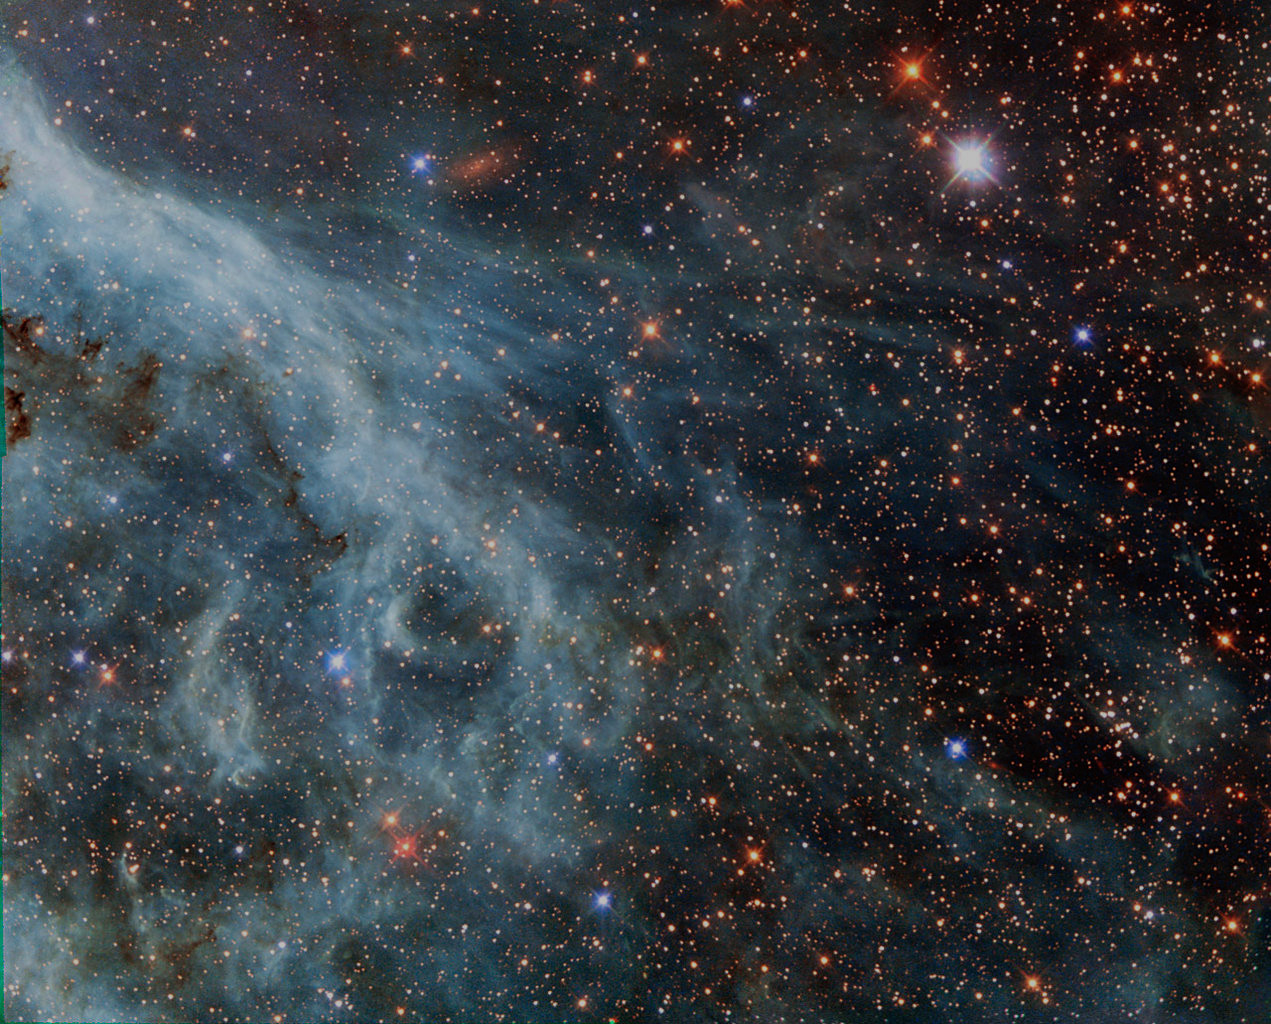
\includegraphics[width=\paperwidth,height=\paperheight]{../common/bg_galaxy.jpg}}
\begin{frame}
\titlepage{}
\end{frame}
}

\begin{frame}[fragile]
\frametitle{What is clang-tidy?}
  It is a \textbf{\textcolor{clTwelveBitOrange}{linter}} tool for C++%
\footnote[frame]{primarily. But C and some other languages are partially supported too},
  based on Clang toolset.
  \begin{itemize}
    \item{} Its purpose is to provide an extensible framework for diagnosing and fixing programming errors,
            like style violations, interface misuse, or bugs that can be deduced via static analysis.
    \item{} greatly customizable
    \item{} setup once (per project), write more correct code forever.
  \end{itemize}
  \vspace*{24pt}
  {\fontsize{9}{9} \url{https://releases.llvm.org/6.0.0/tools/clang/tools/extra/docs/clang-tidy/index.html}}
\end{frame}

\begin{frame}[fragile]
\frametitle{Installing Clang-Tidy on target system}
  Clang-Tidy is already packaged by most popular Linux distributions.
  \begin{itemize}
    \item{} Debian/Ubuntu
    {\fontsize{8}{6} \begin{lstlisting}[showstringspaces=false]
sudo apt-get install clang-tidy
    \end{lstlisting}}
  \end{itemize}
  \vspace*{6pt}

  Clang-Tidy is also part of Clang toolset
  \begin{itemize}
    \item{} Arch Linux
    {\fontsize{8}{6} \begin{lstlisting}[showstringspaces=false]
sudo pacman -S clang
    \end{lstlisting}}
      {\fontsize{8}{6} \url{https://archlinux.org/packages/extra/x86_64/clang/files/}}
  \end{itemize}
  \vspace*{6pt}

  Or provided by clang-tools-extra
  \begin{itemize}
    \item{} Fedora 29
    {\fontsize{8}{6} \begin{lstlisting}[showstringspaces=false]
sudo dnf install clang-tools-extra
    \end{lstlisting}}
  \end{itemize}
  \vspace*{6pt}

  Or one can always build it from source.
\end{frame}

\begin{frame}[fragile]
\frametitle{Getting a list of all available checkers}
  {\fontsize{10}{6} \begin{lstlisting}[showstringspaces=false]
clang-tidy --list-checks -checks='*' | grep "modernize"
    \end{lstlisting}}

\begin{columns}[T]
  \begin{column}{0.5\textwidth}
    {\fontsize{6}{6} \begin{lstlisting}[showstringspaces=false]
      modernize-avoid-bind
      modernize-avoid-c-arrays
      modernize-concat-nested-namespaces
      modernize-deprecated-headers
      modernize-deprecated-ios-base-aliases
      modernize-loop-convert
      modernize-make-shared
      modernize-make-unique
      modernize-pass-by-value
      modernize-raw-string-literal
      modernize-redundant-void-arg
      modernize-replace-auto-ptr
      modernize-replace-disallow-copy-and-assign-macro
      modernize-replace-random-shuffle
      modernize-return-braced-init-list
      modernize-shrink-to-fit
    \end{lstlisting}}
  \end{column}
  \begin{column}{0.5\textwidth}
    {\fontsize{6}{6} \begin{lstlisting}[showstringspaces=false]
modernize-unary-static-assert
modernize-use-auto
modernize-use-bool-literals
modernize-use-default-member-init
modernize-use-emplace
modernize-use-equals-default
modernize-use-equals-delete
modernize-use-nodiscard
modernize-use-noexcept
modernize-use-nullptr
modernize-use-override
modernize-use-trailing-return-type
modernize-use-transparent-functors
modernize-use-uncaught-exceptions
modernize-use-using
    \end{lstlisting}}
  \end{column}
\end{columns}
\end{frame}

\begin{frame}[fragile]
\frametitle{Structure of clang-tidy invocation}
  \hspace*{-12pt}{\large \texttt{\textcolor{clTwelveBitDarkGray}{clang-tidy}
  -checks='\textcolor{clTwelveBitAqua}{*}'
  \textcolor{clTwelveBitRed}{file.cpp}
  \textcolor{clTwelveBitDarkGray}{--} -I\textcolor{clTwelveBitViolet}{src/include}
  -D\textcolor{clTwelveBitViolet}{MY\_DEFINES} ...}}
\end{frame}


\begin{frame}[fragile]
  \frametitle{Let's check \texttt{modernize-use-override} checker!}
  \begin{columns}[T]
    \begin{column}{0.6\textwidth}<1->
      {\color[HTML]{cb4b16}
      \texttt{\textbf{code/my\_game.cpp}}\vspace{-9pt}
      \rule{\linewidth}{2pt}}%
      {\fontsize{7}{6} \lstinputlisting[showstringspaces=false]{code/my_game.cpp}}%
      \vspace{-12pt}{\color[HTML]{cb4b16}\rule{\linewidth}{2pt}}
      \hspace*{160pt}{\small \textcolor{clTwelveBitAqua}{\textit{Spot the problem?}}}
    \end{column}
    \begin{column}{0.4\textwidth}<2->
      Since C++11, one should use \cpp{override} keyword to mark functions in derived classes that override functions defined in the base class.\\
      \vspace*{12pt}%
      But let's have \texttt{clang-tidy} tell us that.\\
      \vspace*{6pt}%

    {\fontsize{6}{6} \begin{lstlisting}[showstringspaces=false]
clang-tidy --checks='modernize-use-override'
           code/my_game.cpp --
    \end{lstlisting}}
    \end{column}
  \end{columns}
\end{frame}


\begin{frame}[fragile]
  \frametitle{Let's check \texttt{modernize-use-override} checker!}
    {\fontsize{8}{6} \begin{lstlisting}[showstringspaces=false]
clang-tidy --checks='modernize-use-override' code/my_game.cpp --
    \end{lstlisting}}
    {\fontsize{6}{6} \begin{lstlisting}[showstringspaces=false]
Error while trying to load a compilation database:
Could not auto-detect compilation database for file "code/my_game.cpp"
No compilation database found in /mnt/vault/Repos/agral/Lectures/CPP_FFFE/26_ClangTidy/code
    or any parent directory
json-compilation-database: Error while opening JSON database: No such file or directory
fixed-compilation-database: Error while opening fixed database: No such file or directory
Running without flags.
90 warnings generated.
/mnt/vault/Repos/agral/Lectures/CPP_FFFE/26_ClangTidy/code/my_game.cpp:13:16: warning:
    prefer using 'override' or (rarely) 'final' instead of 'virtual' [modernize-use-override]

  virtual void draw() {
  ~~~~~~~~     ^
                      override
Suppressed 89 warnings (89 in non-user code).
Use -header-filter=.* to display errors from all non-system headers.
    Use -system-headers to display errors from system headers as well.
    \end{lstlisting}}
  \pause{}
  \vspace*{18pt}
  \begin{center}{\Large OK. Do \textcolor{clTwelveBitGreen}{you} know how to fix it?}\end{center}
    \begin{itemize}
      \item{}Y (\textit{congratulations!})
      \item{}N (\textit{don't worry, it can be \textcolor{clTwelveBitOrange}{fixed automatically}!})
    \end{itemize}
\end{frame}

\begin{frame}[fragile]
  \frametitle{Fixing the indicated problem}
    {\fontsize{8}{6} \begin{lstlisting}[showstringspaces=false]
clang-tidy --checks='modernize-use-override' code/my_game_fixed.cpp -fix --
    \end{lstlisting}}
    {\fontsize{6}{6} \begin{lstlisting}[showstringspaces=false]
Error while trying to load a compilation database:
Could not auto-detect compilation database for file "code/my_game_fixed.cpp"
No compilation database found in /mnt/vault/Repos/agral/Lectures/CPP_FFFE/26_ClangTidy/code or any parent directory
json-compilation-database: Error while opening JSON database: No such file or directory
fixed-compilation-database: Error while opening fixed database: No such file or directory
Running without flags.
90 warnings generated.
/mnt/vault/Repos/agral/Lectures/CPP_FFFE/26_ClangTidy/code/my_game_fixed.cpp:13:16: warning: prefer using 'override' or (rarely) 'final' instead of 'virtual' [modernize-use-override]
  virtual void draw() {
  ~~~~~~~~     ^
                      override
/mnt/vault/Repos/agral/Lectures/CPP_FFFE/26_ClangTidy/code/my_game_fixed.cpp:13:3: note: FIX-IT applied suggested code changes
  virtual void draw() {
  ^
/mnt/vault/Repos/agral/Lectures/CPP_FFFE/26_ClangTidy/code/my_game_fixed.cpp:13:22: note: FIX-IT applied suggested code changes
  virtual void draw() {
                     ^
clang-tidy applied 2 of 2 suggested fixes.
Suppressed 89 warnings (89 in non-user code).
Use -header-filter=.* to display errors from all non-system headers. Use -system-headers to display errors from system headers as well.
    \end{lstlisting}}
\end{frame}

\begin{frame}[fragile]
  \frametitle{Fixing the indicated problem}
  \begin{columns}[T]
    \begin{column}{0.5\textwidth}
      \color{clTwelveBitGreen}{%
      \texttt{\textbf{before}}\vspace*{-9pt}
      \rule{\linewidth}{2pt}}\vspace*{-9pt}%
    {\fontsize{7}{6} \color{black}{\lstinputlisting[showstringspaces=false]{code/my_game.cpp}}}%
      \vspace{-12pt}{\color{clTwelveBitGreen}\rule{\linewidth}{2pt}}
    \end{column}

    \begin{column}{0.5\textwidth}
      \color{clTwelveBitViolet}{%
      \texttt{\textbf{after}}\vspace*{-9pt}
      \rule{\linewidth}{2pt}}\vspace*{-9pt}%
    {\fontsize{7}{6} \color{black}{\lstinputlisting[showstringspaces=false]{code/my_game_fixed.cpp}}}%
      \vspace{-12pt}{\color{clTwelveBitViolet}\rule{\linewidth}{2pt}}
    \end{column}
  \end{columns}
\end{frame}

\begin{frame}
\frametitle{Key takeaways}
{\centering
\begin{itemize}
  \item{} You are probably already using it.
  \item{} If you don't, \textit{start using it}.
  \item{} \cpp{modernize-*} checks especially useful in legacy codebases.
\end{itemize}

\vspace{2ex}
\begin{center}{\Large Thank you!}\end{center}
}
\end{frame}

%%%%

\end{document}
